\documentclass{oblivoir}
\usepackage{amsmath,amssymb,amsthm,kotex,mdframed,paralist,kswrapfig}

\newcounter{num}
\newcommand{\prob}
{\bigskip\noindent\refstepcounter{num}\textbf{문제 \arabic{num})}\par}


\newcommand{\ans}{{\raggedleft\textbf{답 : (\qquad\qquad\qquad\qquad\qquad\qquad)}
\par}}

%%%
\begin{document}
\Large

\title{승재 09 - 6학년 2학기 - 02}
\author{}
\date{\today}
\maketitle
%\tableofcontents

\newpage

%
\prob
한 시간에 3분씩 늦어지는 시계가 있습니다. 오늘 오전 10시에 시계를 정확히 맞추었다면 오늘 오후 3시에 이 시계가 가리키는 시각은 오후 몇 시 몇 분입니까?
\par\ans
\bigskip\bigskip

\prob
한 시간에 2분씩 빨라지는 시계가 있습니다. 오늘 오전 7시에 시계를 정확히 맞추었다면 오늘 오후 3시에 이 시계가 가리키는 시각은 오후 몇 시 몇 분입니까?
\par\ans
\bigskip\bigskip

\prob
하루에 30분씩 느려지는 시계가 있습니다. 오늘 정오에 시계를 정확히 맞추었다면 일주일 후 정오에 시계가 가리키는 시각은 몇 시 몇 분입니까?
\par\ans
\bigskip\bigskip

\prob
일정한 속도로 빨라지거나 느려지는 시계가 있습니다.
오늘 오후 1시에 시계를 정확히 맞추었는데 오늘 오후 9시에 9시 32분을 가리키고 있었습니다.
이 시계는 빨라지는 시계입니까? 아니면 느려지는 시계입니까? 그리고 얼마나 빨라지거나 느려집니까?
{\par\raggedleft\textbf{
답 : 시계는 한 시간에 (\qquad\qquad)분 (빨라집니다, 느려집니다.)}
\par}
\newpage

\prob
쌓기나무로 쌓은 모양을 위, 앞, 옆에서 본 그림입니다.
쌓은 쌓기나무가 가장 적은 경우와 가장 많은 경우의 쌓기나무 수는 각각 몇 개입니까?
\begin{figure}[h]
\centering
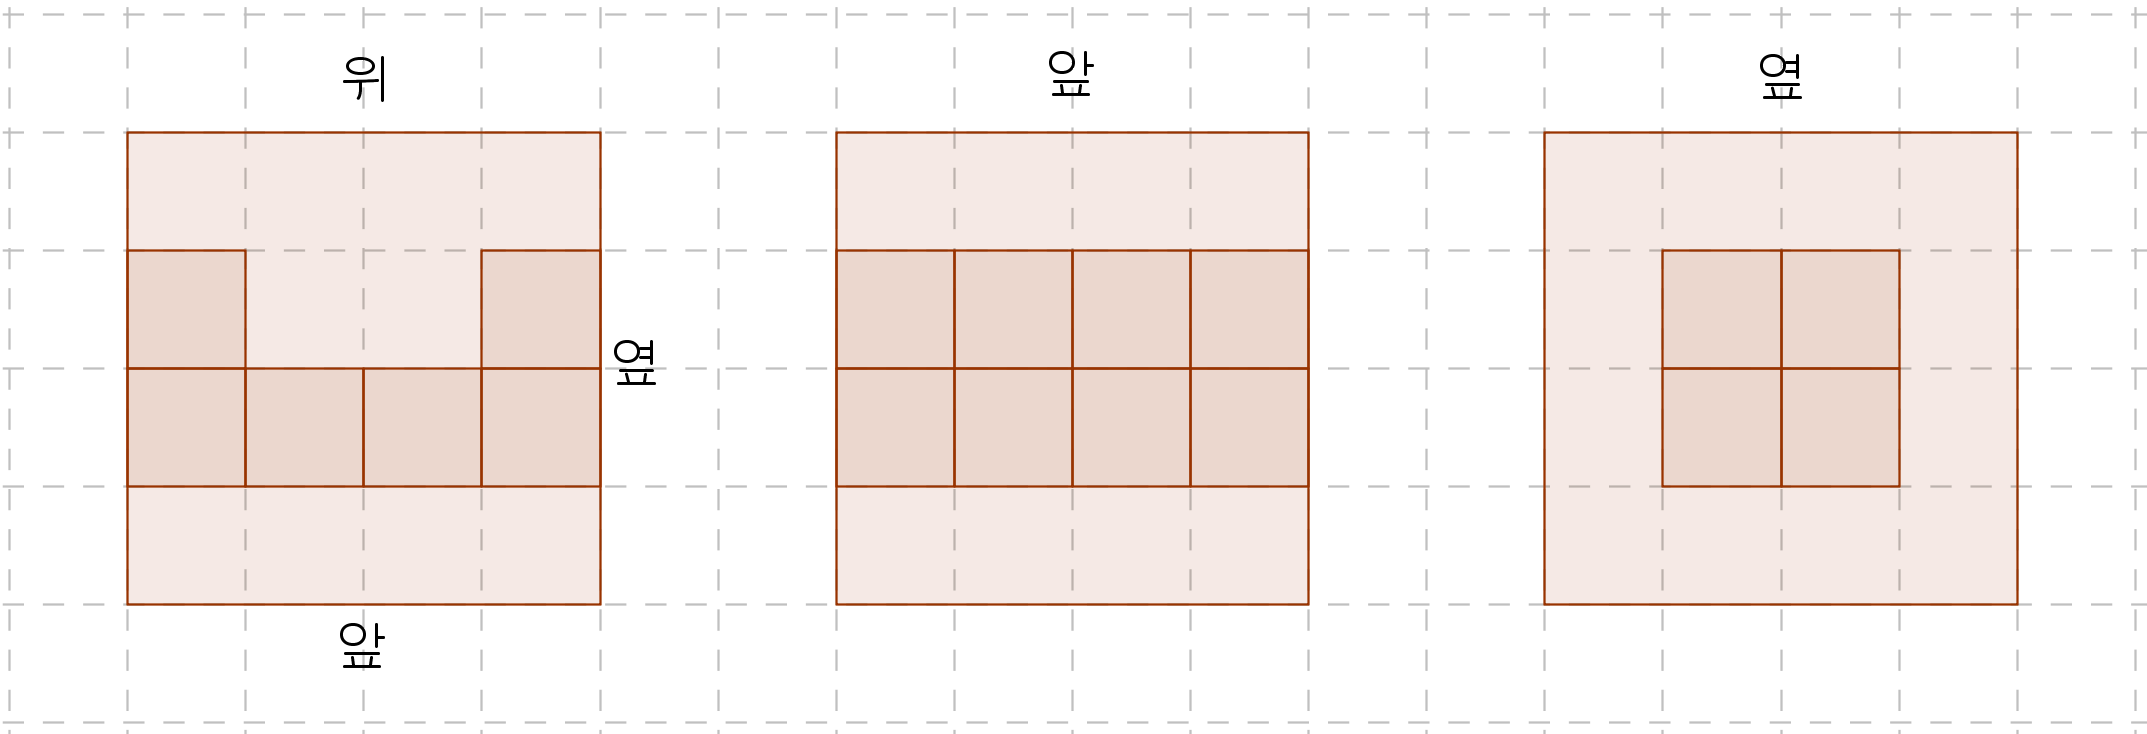
\includegraphics[width=\textwidth]{05}
\end{figure}
{\par\raggedleft\textbf{
가장 적은 경우 : (\qquad\qquad)개\\
가장 많은 경우 : (\qquad\qquad)개}\par}

\prob
문제 5)에서 쌓기나무가 가장 적은 경우의 겉넓이는 얼마입니까?
그리고 가장 많은 경우의 겉넓이는 얼마입니까?
{\par\raggedleft\textbf{
가장 적은 경우 : (\qquad\qquad)cm\(^2\)\\
가장 많은 경우 : (\qquad\qquad)cm\(^2\)}\par}

\newpage

\prob
쌓기나무로 쌓은 모양을 위, 앞, 옆에서 본 그림입니다.
쌓은 쌓기나무가 쌓기나무가 가장 적은 경우의 겉넓이는 얼마입니까?
그리고 가장 많은 경우의 겉넓이는 얼마입니까?
\begin{figure}[h]
\centering
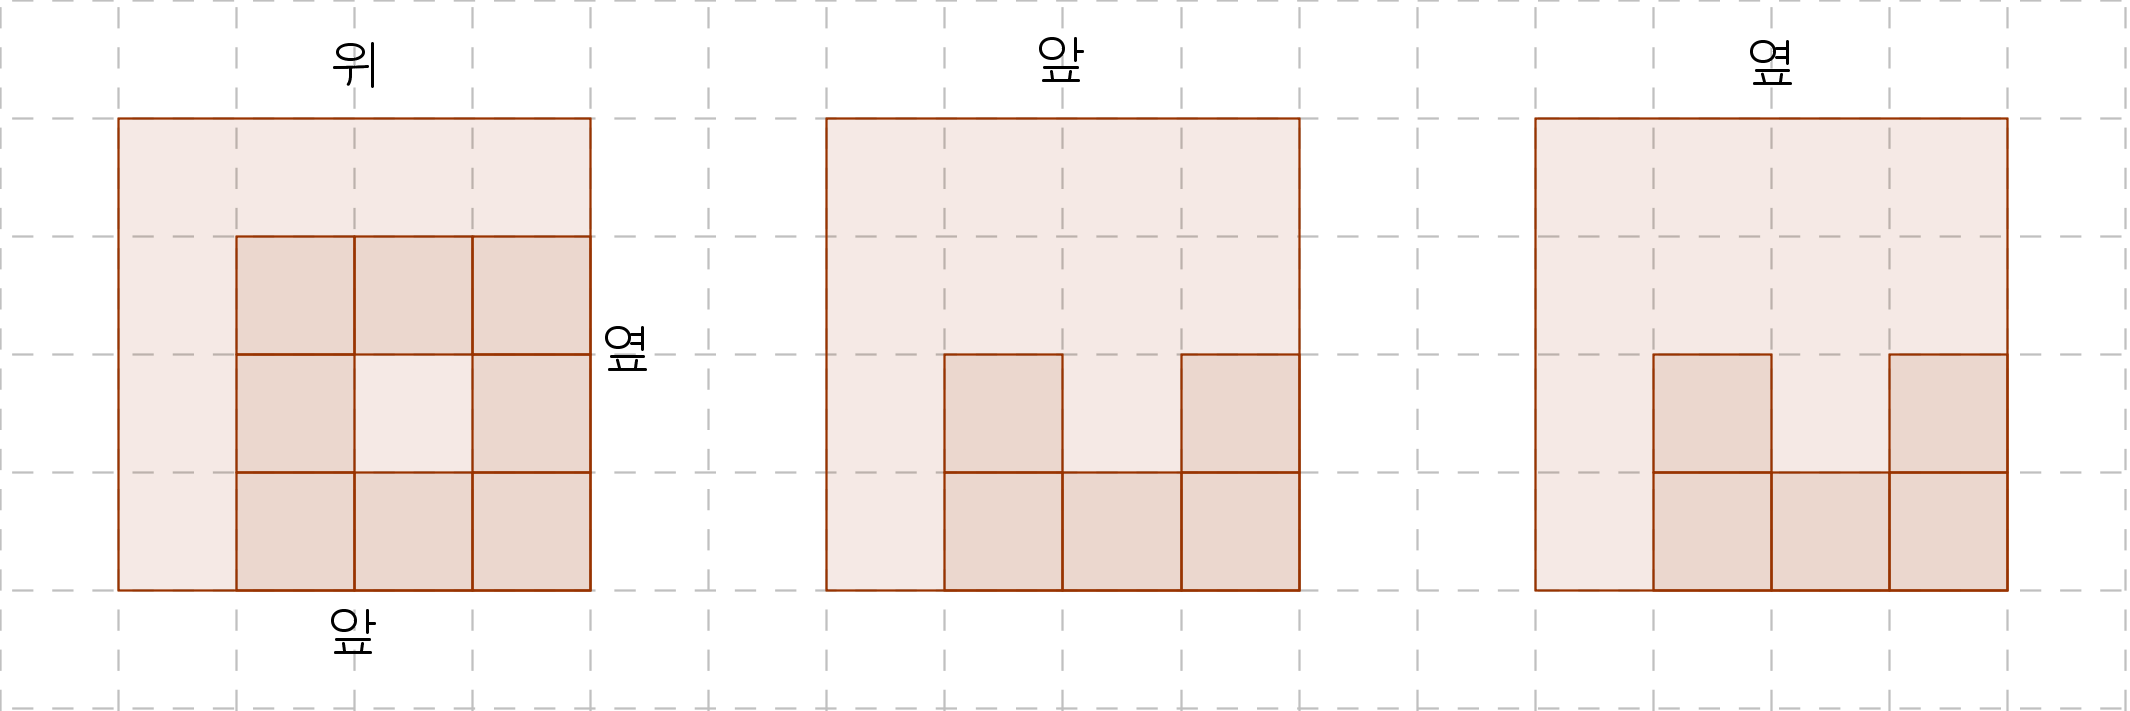
\includegraphics[width=\textwidth]{07}
\end{figure}
{\par\raggedleft\textbf{
가장 적은 경우 : (\qquad\qquad)cm\(^2\)\\
가장 많은 경우 : (\qquad\qquad)cm\(^2\)}\par}

\prob
쌓기나무로 쌓은 모양을 위, 앞, 옆에서 본 그림입니다.
쌓은 쌓기나무가 쌓기나무가 가장 적은 경우의 겉넓이는 얼마입니까?
그리고 가장 많은 경우의 겉넓이는 얼마입니까?
\begin{figure}[h]
\centering
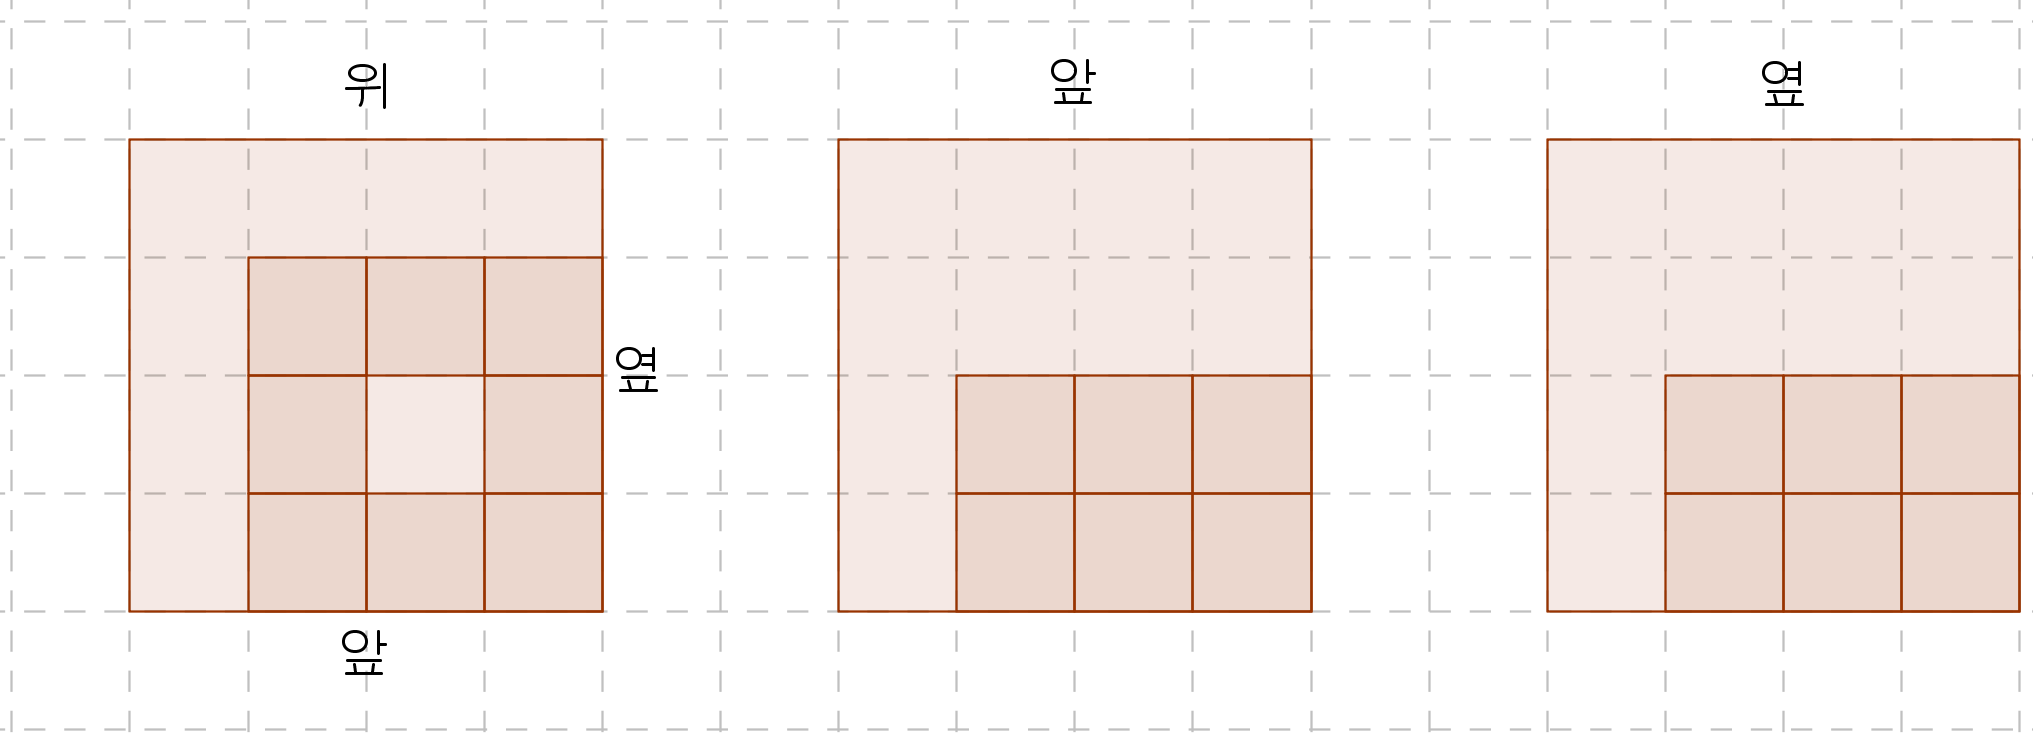
\includegraphics[width=\textwidth]{08}
\end{figure}
{\par\raggedleft\textbf{
가장 적은 경우 : (\qquad\qquad)cm\(^2\)\\
가장 많은 경우 : (\qquad\qquad)cm\(^2\)}\par}

\newpage

\prob
아래 그림은 한 변이 1cm인 쌓기나무로 쌓은 모양입니다.
쌓은 모양의 겉넓이는 몇 cm\(^2\)입니까?
\begin{figure}[h]
\centering
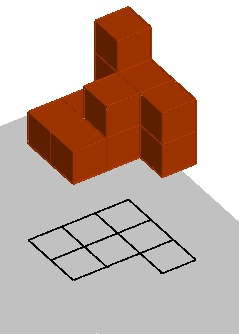
\includegraphics[width=0.35\textwidth]{09}
\end{figure}
{\par\raggedleft\textbf{
답 : (\qquad\qquad\qquad\qquad\qquad)cm\(^2\)}
\par}

\prob
아래 그림은 한 변이 1cm인 쌓기나무로 쌓은 모양입니다.
쌓은 모양의 겉넓이는 몇 cm\(^2\)입니까?
\begin{figure}[h]
\centering
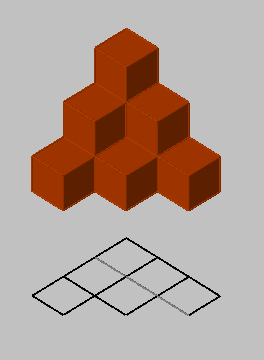
\includegraphics[width=0.35\textwidth]{10}
\end{figure}
{\par\raggedleft\textbf{
답 : (\qquad\qquad\qquad\qquad\qquad)cm\(^2\)}
\par}

\newpage

\prob
다음과 같은 평행사변형을 넓이의 비가 3:1이 되도록 도형 `가'와 도형 `나'로 나누려고 합니다.
도형 `나'의 밑변은 몇 cm\(^2\)입니까?

\begin{figure}[h]
\centering
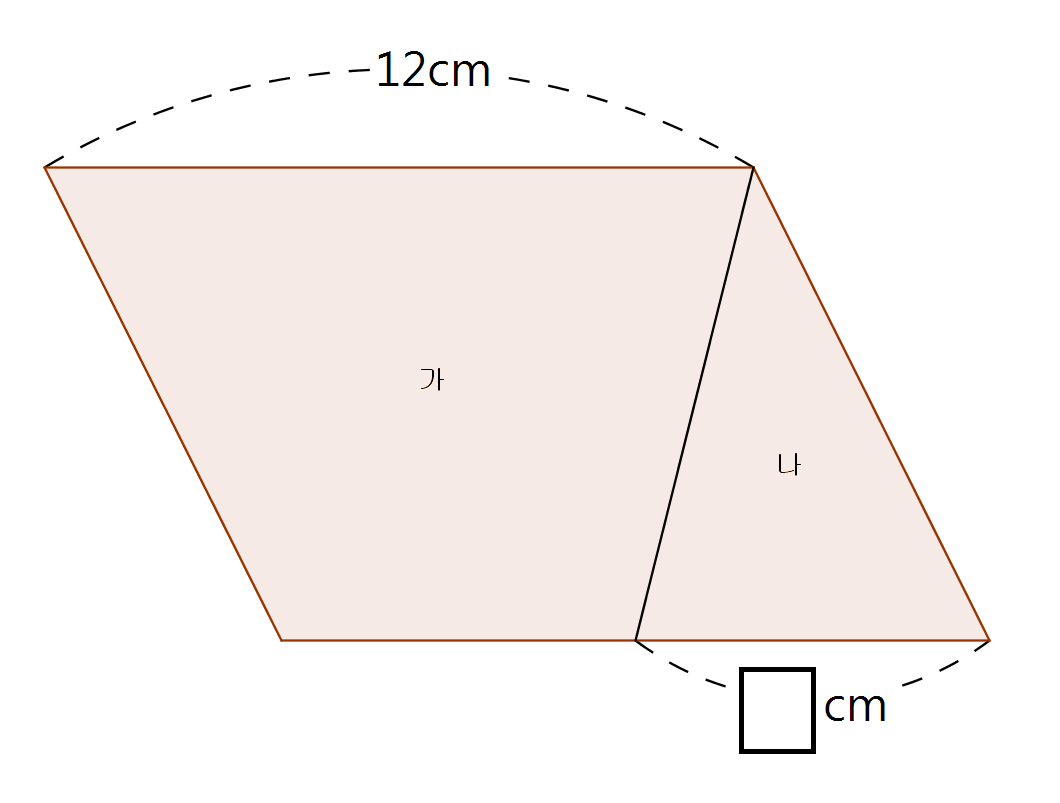
\includegraphics[width=0.6\textwidth]{11}
\end{figure}
\ans

\prob
다음과 같은 직사각형을 넓이의 비가 6:1이 되도록 도형 `가'와 도형 `나'로 나누려고 합니다.
도형 `나'의 밑변은 몇 cm\(^2\)입니까?

\begin{figure}[h]
\centering
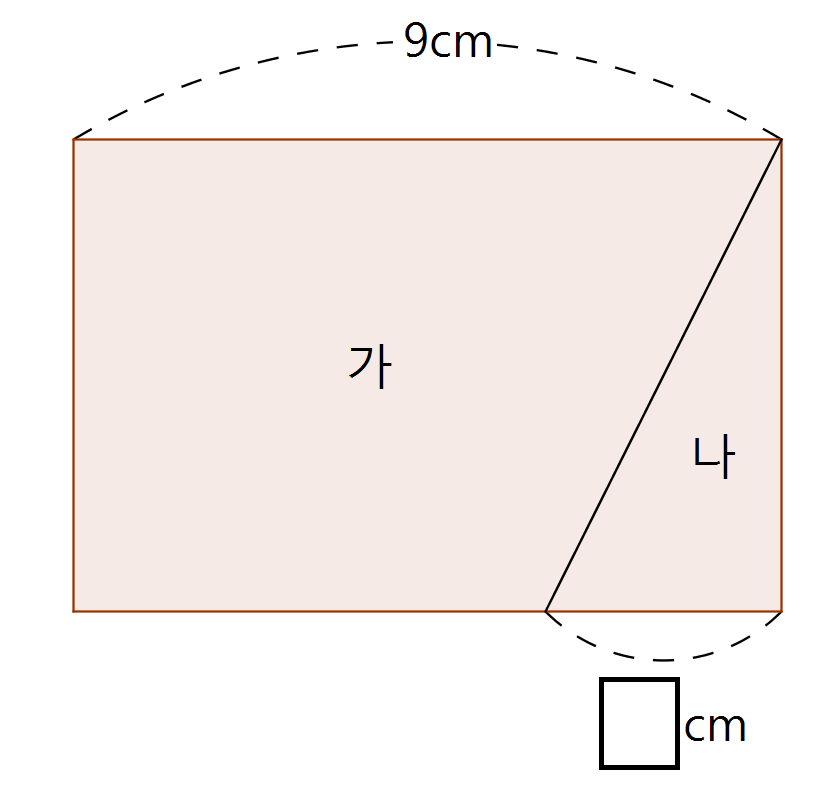
\includegraphics[width=0.5\textwidth]{12}
\end{figure}
\ans

\newpage

\prob
직선 `가'와 `나'가 서로 평행할 때, 도형 `A'와 도형 `B'의 넓이의 비를 가장 간단한 자연수의 비로 나타내세요.

\begin{figure}[h]
\centering
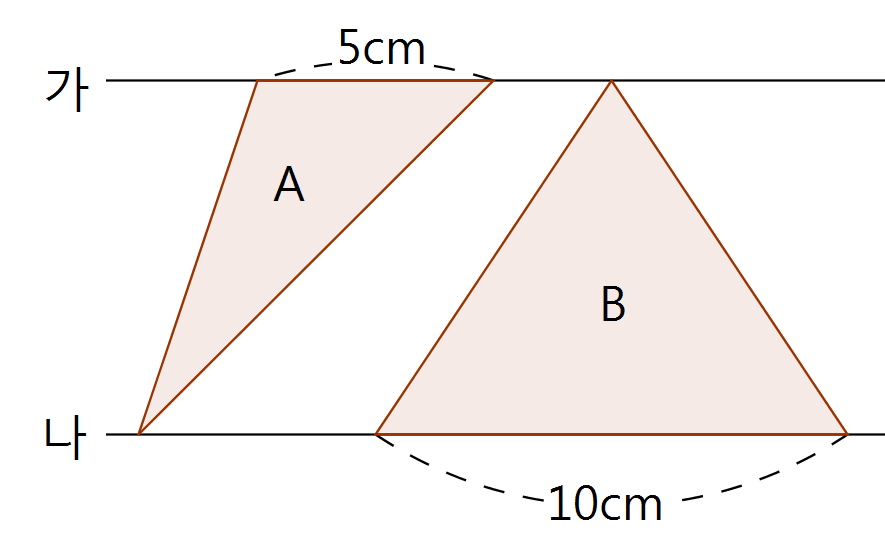
\includegraphics[width=0.5\textwidth]{13}
\end{figure}
\ans

\prob
직선 `가'와 `나'가 서로 평행할 때, 도형 `A'와 도형 `B'의 넓이의 비가 2:3입니다.
B의 밑면의 길이는 몇 cm입니까?

\begin{figure}[h]
\centering
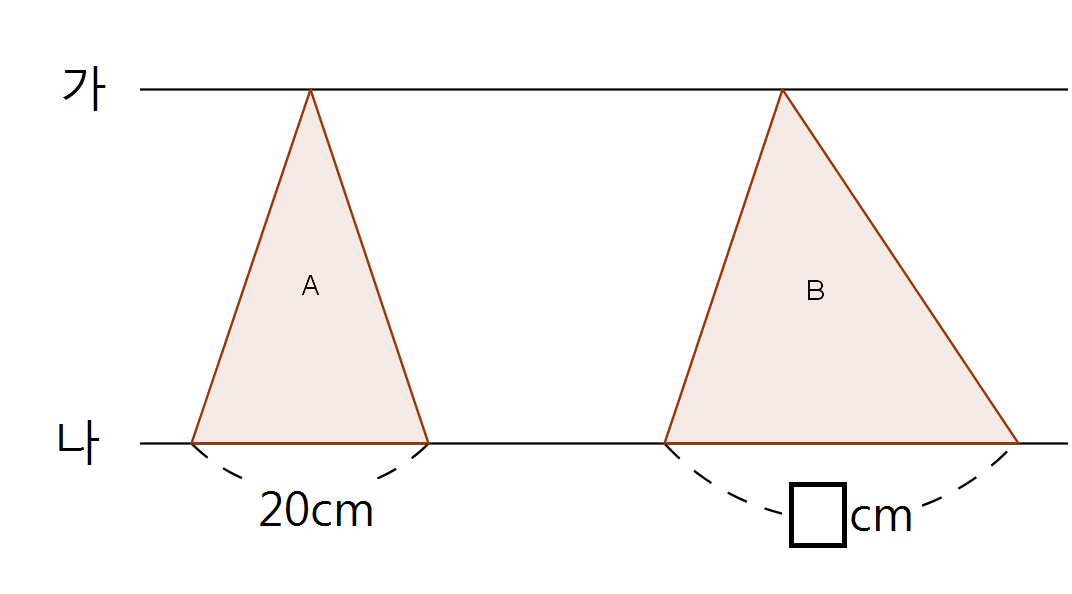
\includegraphics[width=0.5\textwidth]{14}
\end{figure}
\ans
\end{document}